\documentclass[twoside]{book}

% Packages required by doxygen
\usepackage{fixltx2e}
\usepackage{calc}
\usepackage{doxygen}
\usepackage[export]{adjustbox} % also loads graphicx
\usepackage{graphicx}
\usepackage[utf8]{inputenc}
\usepackage{makeidx}
\usepackage{multicol}
\usepackage{multirow}
\PassOptionsToPackage{warn}{textcomp}
\usepackage{textcomp}
\usepackage[nointegrals]{wasysym}
\usepackage[table]{xcolor}

% Font selection
\usepackage[T1]{fontenc}
\usepackage[scaled=.90]{helvet}
\usepackage{courier}
\usepackage{amssymb}
\usepackage{sectsty}
\renewcommand{\familydefault}{\sfdefault}
\allsectionsfont{%
  \fontseries{bc}\selectfont%
  \color{darkgray}%
}
\renewcommand{\DoxyLabelFont}{%
  \fontseries{bc}\selectfont%
  \color{darkgray}%
}
\newcommand{\+}{\discretionary{\mbox{\scriptsize$\hookleftarrow$}}{}{}}

% Page & text layout
\usepackage{geometry}
\geometry{%
  a4paper,%
  top=2.5cm,%
  bottom=2.5cm,%
  left=2.5cm,%
  right=2.5cm%
}
\tolerance=750
\hfuzz=15pt
\hbadness=750
\setlength{\emergencystretch}{15pt}
\setlength{\parindent}{0cm}
\setlength{\parskip}{3ex plus 2ex minus 2ex}
\makeatletter
\renewcommand{\paragraph}{%
  \@startsection{paragraph}{4}{0ex}{-1.0ex}{1.0ex}{%
    \normalfont\normalsize\bfseries\SS@parafont%
  }%
}
\renewcommand{\subparagraph}{%
  \@startsection{subparagraph}{5}{0ex}{-1.0ex}{1.0ex}{%
    \normalfont\normalsize\bfseries\SS@subparafont%
  }%
}
\makeatother

% Headers & footers
\usepackage{fancyhdr}
\pagestyle{fancyplain}
\fancyhead[LE]{\fancyplain{}{\bfseries\thepage}}
\fancyhead[CE]{\fancyplain{}{}}
\fancyhead[RE]{\fancyplain{}{\bfseries\leftmark}}
\fancyhead[LO]{\fancyplain{}{\bfseries\rightmark}}
\fancyhead[CO]{\fancyplain{}{}}
\fancyhead[RO]{\fancyplain{}{\bfseries\thepage}}
\fancyfoot[LE]{\fancyplain{}{}}
\fancyfoot[CE]{\fancyplain{}{}}
\fancyfoot[RE]{\fancyplain{}{\bfseries\scriptsize Generated by Doxygen }}
\fancyfoot[LO]{\fancyplain{}{\bfseries\scriptsize Generated by Doxygen }}
\fancyfoot[CO]{\fancyplain{}{}}
\fancyfoot[RO]{\fancyplain{}{}}
\renewcommand{\footrulewidth}{0.4pt}
\renewcommand{\chaptermark}[1]{%
  \markboth{#1}{}%
}
\renewcommand{\sectionmark}[1]{%
  \markright{\thesection\ #1}%
}

% Indices & bibliography
\usepackage{natbib}
\usepackage[titles]{tocloft}
\setcounter{tocdepth}{3}
\setcounter{secnumdepth}{5}
\makeindex

% Hyperlinks (required, but should be loaded last)
\usepackage{ifpdf}
\ifpdf
  \usepackage[pdftex,pagebackref=true]{hyperref}
\else
  \usepackage[ps2pdf,pagebackref=true]{hyperref}
\fi
\hypersetup{%
  colorlinks=true,%
  linkcolor=blue,%
  citecolor=blue,%
  unicode%
}

% Custom commands
\newcommand{\clearemptydoublepage}{%
  \newpage{\pagestyle{empty}\cleardoublepage}%
}

\usepackage{caption}
\captionsetup{labelsep=space,justification=centering,font={bf},singlelinecheck=off,skip=4pt,position=top}

%===== C O N T E N T S =====

\begin{document}

% Titlepage & ToC
\hypersetup{pageanchor=false,
             bookmarksnumbered=true,
             pdfencoding=unicode
            }
\pagenumbering{alph}
\begin{titlepage}
\vspace*{7cm}
\begin{center}%
{\Large Ohm -\/ Desktop Version \\[1ex]\large 1.\+0 }\\
\vspace*{1cm}
{\large Generated by Doxygen 1.8.12}\\
\end{center}
\end{titlepage}
\clearemptydoublepage
\pagenumbering{roman}
\tableofcontents
\clearemptydoublepage
\pagenumbering{arabic}
\hypersetup{pageanchor=true}

%--- Begin generated contents ---
\chapter{Module Index}
\section{Modules}
Here is a list of all modules\+:\begin{DoxyCompactList}
\item \contentsline{section}{User\+Interface}{\pageref{group___user_interface}}{}
\item \contentsline{section}{Colour\+Mapping}{\pageref{group___colour_mapping}}{}
\item \contentsline{section}{Value\+Calculator}{\pageref{group___value_calculator}}{}
\item \contentsline{section}{Band\+Location}{\pageref{group___band_location}}{}
\item \contentsline{section}{Resistor\+ID}{\pageref{group___resistor_i_d}}{}
\item \contentsline{section}{Camera\+Input}{\pageref{group___camera_input}}{}
\item \contentsline{section}{Image\+Input}{\pageref{group___image_input}}{}
\end{DoxyCompactList}

\chapter{Namespace Index}
\section{Packages}
Here are the packages with brief descriptions (if available)\+:\begin{DoxyCompactList}
\item\contentsline{section}{\hyperlink{namespaceimageprocessing}{imageprocessing} }{\pageref{namespaceimageprocessing}}{}
\item\contentsline{section}{\hyperlink{namespaceinput}{input} }{\pageref{namespaceinput}}{}
\item\contentsline{section}{\hyperlink{namespace_user_interface}{User\+Interface} }{\pageref{namespace_user_interface}}{}
\item\contentsline{section}{\hyperlink{namespacevalueidentification}{valueidentification} }{\pageref{namespacevalueidentification}}{}
\end{DoxyCompactList}

\chapter{Hierarchical Index}
\section{Class Hierarchy}
This inheritance list is sorted roughly, but not completely, alphabetically\+:\begin{DoxyCompactList}
\item \contentsline{section}{ohm.\+Image\+Processing.\+Band\+Reader}{\pageref{classohm_1_1_image_processing_1_1_band_reader}}{}
\item \contentsline{section}{ohm.\+Helpers}{\pageref{classohm_1_1_helpers}}{}
\item \contentsline{section}{ohm.\+Input.\+Input}{\pageref{interfaceohm_1_1_input_1_1_input}}{}
\begin{DoxyCompactList}
\item \contentsline{section}{ohm.\+Input.\+Camera\+Input}{\pageref{classohm_1_1_input_1_1_camera_input}}{}
\item \contentsline{section}{ohm.\+Input.\+Image\+Input}{\pageref{classohm_1_1_input_1_1_image_input}}{}
\end{DoxyCompactList}
\item \contentsline{section}{ohm.\+Image\+Processing.\+Ohm\+Image\+Processor}{\pageref{classohm_1_1_image_processing_1_1_ohm_image_processor}}{}
\item \contentsline{section}{ohm.\+Image\+Processing.\+Resistor\+Body\+ID}{\pageref{classohm_1_1_image_processing_1_1_resistor_body_i_d}}{}
\item \contentsline{section}{ohm.\+Value\+Identification.\+Resistor\+Colour}{\pageref{enumohm_1_1_value_identification_1_1_resistor_colour}}{}
\item \contentsline{section}{ohm.\+Value\+Identification.\+Value\+Calculator}{\pageref{classohm_1_1_value_identification_1_1_value_calculator}}{}
\item Application\begin{DoxyCompactList}
\item \contentsline{section}{ohm.\+Ohm}{\pageref{classohm_1_1_ohm}}{}
\end{DoxyCompactList}
\item Event\+Handler\begin{DoxyCompactList}
\item \contentsline{section}{ohm.\+userinterface.\+Resistor\+Axis\+Picker\+View}{\pageref{classohm_1_1userinterface_1_1_resistor_axis_picker_view}}{}
\end{DoxyCompactList}
\item Image\+View\begin{DoxyCompactList}
\item \contentsline{section}{ohm.\+userinterface.\+Live\+Image\+View}{\pageref{classohm_1_1userinterface_1_1_live_image_view}}{}
\item \contentsline{section}{ohm.\+userinterface.\+Resistor\+Axis\+Picker\+View}{\pageref{classohm_1_1userinterface_1_1_resistor_axis_picker_view}}{}
\end{DoxyCompactList}
\item Initializable\begin{DoxyCompactList}
\item \contentsline{section}{ohm.\+userinterface.\+Ohm\+View\+Controller}{\pageref{classohm_1_1userinterface_1_1_ohm_view_controller}}{}
\end{DoxyCompactList}
\end{DoxyCompactList}

\chapter{Class Index}
\section{Class List}
Here are the classes, structs, unions and interfaces with brief descriptions\+:\begin{DoxyCompactList}
\item\contentsline{section}{\hyperlink{classohm_1_1_image_processing_1_1_band_reader}{ohm.\+Image\+Processing.\+Band\+Reader} \\*Module used to analyze the line of pixels selected by the user through the UI. It uses high values of the differential of the R\+GB colours to detect edges of bands }{\pageref{classohm_1_1_image_processing_1_1_band_reader}}{}
\item\contentsline{section}{\hyperlink{classohm_1_1_input_1_1_camera_input}{ohm.\+Input.\+Camera\+Input} \\*Instances of this class are to be used to receive input from device camera. Currently unimplemented }{\pageref{classohm_1_1_input_1_1_camera_input}}{}
\item\contentsline{section}{\hyperlink{classohm_1_1_helpers}{ohm.\+Helpers} }{\pageref{classohm_1_1_helpers}}{}
\item\contentsline{section}{\hyperlink{classohm_1_1_input_1_1_image_input}{ohm.\+Input.\+Image\+Input} \\*A source of input data, uses static images }{\pageref{classohm_1_1_input_1_1_image_input}}{}
\item\contentsline{section}{\hyperlink{interfaceohm_1_1_input_1_1_input}{ohm.\+Input.\+Input} }{\pageref{interfaceohm_1_1_input_1_1_input}}{}
\item\contentsline{section}{\hyperlink{classohm_1_1userinterface_1_1_live_image_view}{ohm.\+userinterface.\+Live\+Image\+View} \\*The \hyperlink{classohm_1_1userinterface_1_1_live_image_view}{Live\+Image\+View} is an Image\+View that periodically calls a Renderer to produce a new image that the Image\+View then displays. This is useful to create images from real time updating images/data }{\pageref{classohm_1_1userinterface_1_1_live_image_view}}{}
\item\contentsline{section}{\hyperlink{classohm_1_1_ohm}{ohm.\+Ohm} }{\pageref{classohm_1_1_ohm}}{}
\item\contentsline{section}{\hyperlink{classohm_1_1_image_processing_1_1_ohm_image_processor}{ohm.\+Image\+Processing.\+Ohm\+Image\+Processor} \\*Module that will be used as a means of combining the algorithms outlined in \hyperlink{classohm_1_1_image_processing_1_1_band_reader}{Band\+Reader} and \hyperlink{classohm_1_1_image_processing_1_1_resistor_body_i_d}{Resistor\+Body\+ID}. Not yet implemented }{\pageref{classohm_1_1_image_processing_1_1_ohm_image_processor}}{}
\item\contentsline{section}{\hyperlink{classohm_1_1userinterface_1_1_ohm_view_controller}{ohm.\+userinterface.\+Ohm\+View\+Controller} \\*Coordinates the algorithms present in the model with user input through the view }{\pageref{classohm_1_1userinterface_1_1_ohm_view_controller}}{}
\item\contentsline{section}{\hyperlink{classohm_1_1userinterface_1_1_resistor_axis_picker_view}{ohm.\+userinterface.\+Resistor\+Axis\+Picker\+View} \\*This class displays an opencv Mat as an image and allows the user to pick two endpoints of a line. Once two valid points, a listener is called }{\pageref{classohm_1_1userinterface_1_1_resistor_axis_picker_view}}{}
\item\contentsline{section}{\hyperlink{classohm_1_1_image_processing_1_1_resistor_body_i_d}{ohm.\+Image\+Processing.\+Resistor\+Body\+ID} }{\pageref{classohm_1_1_image_processing_1_1_resistor_body_i_d}}{}
\item\contentsline{section}{\hyperlink{enumohm_1_1_value_identification_1_1_resistor_colour}{ohm.\+Value\+Identification.\+Resistor\+Colour} \\*Enum containing all of the possible colours that a resistor can take on. Also features member functions used to map the colours of bands to values used in the calculation process }{\pageref{enumohm_1_1_value_identification_1_1_resistor_colour}}{}
\end{DoxyCompactList}

\chapter{Module Documentation}
\hypertarget{group___user_interface}{}\section{User\+Interface}
\label{group___user_interface}\index{User\+Interface@{User\+Interface}}
\subsection*{Classes}
\begin{DoxyCompactItemize}
\item 
class \hyperlink{classohm_1_1userinterface_1_1_live_image_view}{ohm.\+userinterface.\+Live\+Image\+View}
\begin{DoxyCompactList}\small\item\em The \hyperlink{classohm_1_1userinterface_1_1_live_image_view}{Live\+Image\+View} is an Image\+View that periodically calls a Renderer to produce a new image that the Image\+View then displays. This is useful to create images from real time updating images/data. \end{DoxyCompactList}\item 
class \hyperlink{classohm_1_1userinterface_1_1_ohm_view_controller}{ohm.\+userinterface.\+Ohm\+View\+Controller}
\begin{DoxyCompactList}\small\item\em Coordinates the algorithms present in the model with user input through the view. \end{DoxyCompactList}\item 
class \hyperlink{classohm_1_1userinterface_1_1_resistor_axis_picker_view}{ohm.\+userinterface.\+Resistor\+Axis\+Picker\+View}
\begin{DoxyCompactList}\small\item\em This class displays an opencv Mat as an image and allows the user to pick two endpoints of a line. Once two valid points, a listener is called. \end{DoxyCompactList}\end{DoxyCompactItemize}


\subsection{Detailed Description}

\hypertarget{group___colour_mapping}{}\section{Colour\+Mapping}
\label{group___colour_mapping}\index{Colour\+Mapping@{Colour\+Mapping}}
\subsection*{Classes}
\begin{DoxyCompactItemize}
\item 
enum \hyperlink{enumohm_1_1valueidentification_1_1_resistor_colour}{ohm.\+valueidentification.\+Resistor\+Colour}
\begin{DoxyCompactList}\small\item\em Enum containing all of the possible colours that a resistor can take on. Also features member functions used to map the colours of bands to values used in the calculation process. \end{DoxyCompactList}\end{DoxyCompactItemize}


\subsection{Detailed Description}
\begin{DoxyAuthor}{Author}
Jonathan Brown 
\end{DoxyAuthor}

\hypertarget{group___value_calculator}{}\section{Value\+Calculator}
\label{group___value_calculator}\index{Value\+Calculator@{Value\+Calculator}}
\subsection*{Classes}
\begin{DoxyCompactItemize}
\item 
class \hyperlink{classohm_1_1valueidentification_1_1_value_calculator}{ohm.\+valueidentification.\+Value\+Calculator}
\begin{DoxyCompactList}\small\item\em Object used to calculate the resistance of the resistor based on the mapped colours. \end{DoxyCompactList}\end{DoxyCompactItemize}


\subsection{Detailed Description}
\begin{DoxyAuthor}{Author}
Jonathan Brown 
\end{DoxyAuthor}

\hypertarget{group___band_location}{}\section{Band\+Location}
\label{group___band_location}\index{Band\+Location@{Band\+Location}}
\subsection*{Classes}
\begin{DoxyCompactItemize}
\item 
class \hyperlink{classca_1_1ryanmarks_1_1ohm_1_1imageprocessing_1_1_band_reader}{ca.\+ryanmarks.\+ohm.\+imageprocessing.\+Band\+Reader}
\begin{DoxyCompactList}\small\item\em Module used to analyze the line of pixels selected by the user through the UI. It uses high values of the differential of the R\+GB colours to detect edges of bands. \end{DoxyCompactList}\end{DoxyCompactItemize}


\subsection{Detailed Description}
Module used to analyze the line of pixels selected by the user through the UI. It uses high values of the differential of the R\+GB colours to detect edges of bands. 
\hypertarget{group___camera_input}{}\section{Camera\+Input}
\label{group___camera_input}\index{Camera\+Input@{Camera\+Input}}
\subsection*{Classes}
\begin{DoxyCompactItemize}
\item 
class \hyperlink{classohm_1_1input_1_1_camera_input}{ohm.\+input.\+Camera\+Input}
\begin{DoxyCompactList}\small\item\em Class used to receive input from the camera on Desktop. \end{DoxyCompactList}\end{DoxyCompactItemize}


\subsection{Detailed Description}
\begin{DoxyAuthor}{Author}
Graeme Crawley 
\end{DoxyAuthor}

\hypertarget{group___image_input}{}\section{Image\+Input}
\label{group___image_input}\index{Image\+Input@{Image\+Input}}
\subsection*{Classes}
\begin{DoxyCompactItemize}
\item 
class \hyperlink{classohm_1_1_input_1_1_image_input}{ohm.\+Input.\+Image\+Input}
\begin{DoxyCompactList}\small\item\em A source of input data, uses static images. \end{DoxyCompactList}\end{DoxyCompactItemize}


\subsection{Detailed Description}

\chapter{Namespace Documentation}
\hypertarget{namespaceimageprocessing}{}\section{Package imageprocessing}
\label{namespaceimageprocessing}\index{imageprocessing@{imageprocessing}}


\subsection{Detailed Description}
Contains the Band Location and Resistor Body Identification modules. 
\hypertarget{namespaceinput}{}\section{Package input}
\label{namespaceinput}\index{input@{input}}


\subsection{Detailed Description}
This package contains the components of the Camera and Image\+File modules. They hide the applications access to the hardware (camera or file system). 
\hypertarget{namespace_user_interface}{}\section{Package User\+Interface}
\label{namespace_user_interface}\index{User\+Interface@{User\+Interface}}


\subsection{Detailed Description}
Contains the views and the controller of the application. This is a Behavioural Module who\textquotesingle{}s secret is the UI components of the application. 
\hypertarget{namespacevalueidentification}{}\section{Package valueidentification}
\label{namespacevalueidentification}\index{valueidentification@{valueidentification}}


\subsection{Detailed Description}
Contains the Colour Mapping and Value Identification Modules 
\chapter{Class Documentation}
\hypertarget{classohm_1_1imageprocessing_1_1_band_reader}{}\section{ohm.\+imageprocessing.\+Band\+Reader Class Reference}
\label{classohm_1_1imageprocessing_1_1_band_reader}\index{ohm.\+imageprocessing.\+Band\+Reader@{ohm.\+imageprocessing.\+Band\+Reader}}


Module used to analyze the line of pixels selected by the user through the UI. It uses high values of the differential of the R\+GB colours to detect edges of bands.  


\subsection*{Static Public Member Functions}
\begin{DoxyCompactItemize}
\item 
static List$<$ Point $>$ \hyperlink{classohm_1_1imageprocessing_1_1_band_reader_a335c53bee0b8cd3f58939bee33ea5a0e}{read} (Mat frame, Point p1, Point p2)
\item 
static double \mbox{[}$\,$\mbox{]}\mbox{[}$\,$\mbox{]} \hyperlink{classohm_1_1imageprocessing_1_1_band_reader_a70bbf2127dd344ecbaf8190526f65d8c}{box\+Sample} (Mat mat, Point start, Point end, int n\+Samples, double box\+Width)
\item 
static double \mbox{[}$\,$\mbox{]}\mbox{[}$\,$\mbox{]} \hyperlink{classohm_1_1imageprocessing_1_1_band_reader_a4197e296bcb749a582d401e171b06964}{rolling\+Average\+Filter} (double\mbox{[}$\,$\mbox{]}\mbox{[}$\,$\mbox{]} \hyperlink{classohm_1_1imageprocessing_1_1_band_reader_aeac10376ede4d964a2e652f001416581}{sample}, int window\+Radius)
\item 
static double \mbox{[}$\,$\mbox{]} \hyperlink{classohm_1_1imageprocessing_1_1_band_reader_a7a65be0d91e263ba95be40a839a1e9dd}{componentwise\+Mean} (double\mbox{[}$\,$\mbox{]}\mbox{[}$\,$\mbox{]} samples)
\item 
static double \mbox{[}$\,$\mbox{]}\mbox{[}$\,$\mbox{]} \hyperlink{classohm_1_1imageprocessing_1_1_band_reader_aeac10376ede4d964a2e652f001416581}{sample} (Mat mat, Point start, Point end, int n\+Samples)
\item 
static double \mbox{[}$\,$\mbox{]}\mbox{[}$\,$\mbox{]} \hyperlink{classohm_1_1imageprocessing_1_1_band_reader_a1482e17c3db23f374ec320d363fffac1}{diff} (double\mbox{[}$\,$\mbox{]}\mbox{[}$\,$\mbox{]} y)
\item 
static double \hyperlink{classohm_1_1imageprocessing_1_1_band_reader_a89a1ca359c7d26536f149c4dcc38cc99}{abmag} (double\mbox{[}$\,$\mbox{]} vect)
\item 
static double \hyperlink{classohm_1_1imageprocessing_1_1_band_reader_a5a853fa56348caf878ed0fc9c7e0ccaa}{mag} (double\mbox{[}$\,$\mbox{]} vect)
\item 
static double \hyperlink{classohm_1_1imageprocessing_1_1_band_reader_a10ab79859262742046ab3b3dda006c60}{dist} (Point p1, Point p2)
\item 
static double \mbox{[}$\,$\mbox{]} \hyperlink{classohm_1_1imageprocessing_1_1_band_reader_af0fe7156595bf275194c8785477ecd71}{group\+Terms} (double\mbox{[}$\,$\mbox{]} terms, int bin\+Size)
\item 
static List$<$ Pair$<$ Integer, Double $>$ $>$ \hyperlink{classohm_1_1imageprocessing_1_1_band_reader_a14e650d56c1f86b422eb2897ed359ade}{find\+Local\+Maxima} (double\mbox{[}$\,$\mbox{]} values)
\item 
static List$<$ Pair$<$ Integer, Double $>$ $>$ \hyperlink{classohm_1_1imageprocessing_1_1_band_reader_ac5c3bd6e24700bc9bcf8d882c044d1b6}{find\+Global\+Maxima} (double\mbox{[}$\,$\mbox{]} values, int n\+Maxima)
\item 
static Point \hyperlink{classohm_1_1imageprocessing_1_1_band_reader_ab6d2dfccd0b44f46dad708ecee256124}{on\+Line} (Point start, Point end, double fraction)
\end{DoxyCompactItemize}


\subsection{Detailed Description}
Module used to analyze the line of pixels selected by the user through the UI. It uses high values of the differential of the R\+GB colours to detect edges of bands. 

\begin{DoxyAuthor}{Author}
Ryan Marks \& Jonathan Brown 
\end{DoxyAuthor}


\subsection{Member Function Documentation}
\hypertarget{classohm_1_1imageprocessing_1_1_band_reader_a89a1ca359c7d26536f149c4dcc38cc99}{}\label{classohm_1_1imageprocessing_1_1_band_reader_a89a1ca359c7d26536f149c4dcc38cc99} 
\index{ohm\+::imageprocessing\+::\+Band\+Reader@{ohm\+::imageprocessing\+::\+Band\+Reader}!abmag@{abmag}}
\index{abmag@{abmag}!ohm\+::imageprocessing\+::\+Band\+Reader@{ohm\+::imageprocessing\+::\+Band\+Reader}}
\subsubsection{\texorpdfstring{abmag()}{abmag()}}
{\footnotesize\ttfamily static double ohm.\+imageprocessing.\+Band\+Reader.\+abmag (\begin{DoxyParamCaption}\item[{double \mbox{[}$\,$\mbox{]}}]{vect }\end{DoxyParamCaption})\hspace{0.3cm}{\ttfamily [static]}}

Calculate the magnitude of a given vector 
\begin{DoxyParams}{Parameters}
{\em vect} & input vector \\
\hline
\end{DoxyParams}
\begin{DoxyReturn}{Returns}
The magnitude of the input vector 
\end{DoxyReturn}
\hypertarget{classohm_1_1imageprocessing_1_1_band_reader_a70bbf2127dd344ecbaf8190526f65d8c}{}\label{classohm_1_1imageprocessing_1_1_band_reader_a70bbf2127dd344ecbaf8190526f65d8c} 
\index{ohm\+::imageprocessing\+::\+Band\+Reader@{ohm\+::imageprocessing\+::\+Band\+Reader}!box\+Sample@{box\+Sample}}
\index{box\+Sample@{box\+Sample}!ohm\+::imageprocessing\+::\+Band\+Reader@{ohm\+::imageprocessing\+::\+Band\+Reader}}
\subsubsection{\texorpdfstring{box\+Sample()}{boxSample()}}
{\footnotesize\ttfamily static double \mbox{[}$\,$\mbox{]}\mbox{[}$\,$\mbox{]} ohm.\+imageprocessing.\+Band\+Reader.\+box\+Sample (\begin{DoxyParamCaption}\item[{Mat}]{mat,  }\item[{Point}]{start,  }\item[{Point}]{end,  }\item[{int}]{n\+Samples,  }\item[{double}]{box\+Width }\end{DoxyParamCaption})\hspace{0.3cm}{\ttfamily [static]}}

This method takes something Ryan made up called a box sample. At n\+Samples points along the line from start to end, a line of samples are take along a line of length box\+Width, normal to and centred on the sampling line 
\begin{DoxyParams}{Parameters}
{\em mat} & The matrix being sampled \\
\hline
{\em start} & The start of the sampling line \\
\hline
{\em end} & The end of the sampling line \\
\hline
{\em n\+Samples} & The number or linear samples to take along the sampling line \\
\hline
{\em box\+Width} & the length of the normal sampling line. \\
\hline
\end{DoxyParams}
\begin{DoxyReturn}{Returns}
An array containing the average rgb values (represented as double\mbox{[}\mbox{]}) in the sampling window. 
\end{DoxyReturn}
\hypertarget{classohm_1_1imageprocessing_1_1_band_reader_a7a65be0d91e263ba95be40a839a1e9dd}{}\label{classohm_1_1imageprocessing_1_1_band_reader_a7a65be0d91e263ba95be40a839a1e9dd} 
\index{ohm\+::imageprocessing\+::\+Band\+Reader@{ohm\+::imageprocessing\+::\+Band\+Reader}!componentwise\+Mean@{componentwise\+Mean}}
\index{componentwise\+Mean@{componentwise\+Mean}!ohm\+::imageprocessing\+::\+Band\+Reader@{ohm\+::imageprocessing\+::\+Band\+Reader}}
\subsubsection{\texorpdfstring{componentwise\+Mean()}{componentwiseMean()}}
{\footnotesize\ttfamily static double \mbox{[}$\,$\mbox{]} ohm.\+imageprocessing.\+Band\+Reader.\+componentwise\+Mean (\begin{DoxyParamCaption}\item[{double}]{samples\mbox{[}$\,$\mbox{]}\mbox{[}$\,$\mbox{]} }\end{DoxyParamCaption})\hspace{0.3cm}{\ttfamily [static]}}

Calculate the mean of an array of vectors. 
\begin{DoxyParams}{Parameters}
{\em samples} & Array of R\+GB vectors represented as double\mbox{[}\mbox{]} \\
\hline
\end{DoxyParams}
\begin{DoxyReturn}{Returns}
The average of all vectors within the input array (represented as a double\mbox{[}\mbox{]}) 
\end{DoxyReturn}
\hypertarget{classohm_1_1imageprocessing_1_1_band_reader_a1482e17c3db23f374ec320d363fffac1}{}\label{classohm_1_1imageprocessing_1_1_band_reader_a1482e17c3db23f374ec320d363fffac1} 
\index{ohm\+::imageprocessing\+::\+Band\+Reader@{ohm\+::imageprocessing\+::\+Band\+Reader}!diff@{diff}}
\index{diff@{diff}!ohm\+::imageprocessing\+::\+Band\+Reader@{ohm\+::imageprocessing\+::\+Band\+Reader}}
\subsubsection{\texorpdfstring{diff()}{diff()}}
{\footnotesize\ttfamily static double \mbox{[}$\,$\mbox{]}\mbox{[}$\,$\mbox{]} ohm.\+imageprocessing.\+Band\+Reader.\+diff (\begin{DoxyParamCaption}\item[{double}]{y\mbox{[}$\,$\mbox{]}\mbox{[}$\,$\mbox{]} }\end{DoxyParamCaption})\hspace{0.3cm}{\ttfamily [static]}}

Take the discrete derivative of a series of vectors. 
\begin{DoxyParams}{Parameters}
{\em y} & A series of vectors \\
\hline
\end{DoxyParams}
\begin{DoxyReturn}{Returns}
y\textquotesingle{}, the derivative of the input represented as a array of vectors (double\mbox{[}\mbox{]}). 
\end{DoxyReturn}
\hypertarget{classohm_1_1imageprocessing_1_1_band_reader_a10ab79859262742046ab3b3dda006c60}{}\label{classohm_1_1imageprocessing_1_1_band_reader_a10ab79859262742046ab3b3dda006c60} 
\index{ohm\+::imageprocessing\+::\+Band\+Reader@{ohm\+::imageprocessing\+::\+Band\+Reader}!dist@{dist}}
\index{dist@{dist}!ohm\+::imageprocessing\+::\+Band\+Reader@{ohm\+::imageprocessing\+::\+Band\+Reader}}
\subsubsection{\texorpdfstring{dist()}{dist()}}
{\footnotesize\ttfamily static double ohm.\+imageprocessing.\+Band\+Reader.\+dist (\begin{DoxyParamCaption}\item[{Point}]{p1,  }\item[{Point}]{p2 }\end{DoxyParamCaption})\hspace{0.3cm}{\ttfamily [static]}}

Calcualte the distance between two points. 
\begin{DoxyParams}{Parameters}
{\em p1} & Point 1. \\
\hline
{\em p2} & Point 2. \\
\hline
\end{DoxyParams}
\begin{DoxyReturn}{Returns}
Distance between p1 and p2. 
\end{DoxyReturn}
\hypertarget{classohm_1_1imageprocessing_1_1_band_reader_ac5c3bd6e24700bc9bcf8d882c044d1b6}{}\label{classohm_1_1imageprocessing_1_1_band_reader_ac5c3bd6e24700bc9bcf8d882c044d1b6} 
\index{ohm\+::imageprocessing\+::\+Band\+Reader@{ohm\+::imageprocessing\+::\+Band\+Reader}!find\+Global\+Maxima@{find\+Global\+Maxima}}
\index{find\+Global\+Maxima@{find\+Global\+Maxima}!ohm\+::imageprocessing\+::\+Band\+Reader@{ohm\+::imageprocessing\+::\+Band\+Reader}}
\subsubsection{\texorpdfstring{find\+Global\+Maxima()}{findGlobalMaxima()}}
{\footnotesize\ttfamily static List$<$Pair$<$Integer,Double$>$ $>$ ohm.\+imageprocessing.\+Band\+Reader.\+find\+Global\+Maxima (\begin{DoxyParamCaption}\item[{double \mbox{[}$\,$\mbox{]}}]{values,  }\item[{int}]{n\+Maxima }\end{DoxyParamCaption})\hspace{0.3cm}{\ttfamily [static]}}

Get the n largest values in a sample/ 
\begin{DoxyParams}{Parameters}
{\em values} & the input signal \\
\hline
{\em n\+Maxima} & The number of maxima to find \\
\hline
\end{DoxyParams}
\begin{DoxyReturn}{Returns}
A list of (index, value) Pairs representing the global maxima in the sample 
\end{DoxyReturn}
\hypertarget{classohm_1_1imageprocessing_1_1_band_reader_a14e650d56c1f86b422eb2897ed359ade}{}\label{classohm_1_1imageprocessing_1_1_band_reader_a14e650d56c1f86b422eb2897ed359ade} 
\index{ohm\+::imageprocessing\+::\+Band\+Reader@{ohm\+::imageprocessing\+::\+Band\+Reader}!find\+Local\+Maxima@{find\+Local\+Maxima}}
\index{find\+Local\+Maxima@{find\+Local\+Maxima}!ohm\+::imageprocessing\+::\+Band\+Reader@{ohm\+::imageprocessing\+::\+Band\+Reader}}
\subsubsection{\texorpdfstring{find\+Local\+Maxima()}{findLocalMaxima()}}
{\footnotesize\ttfamily static List$<$Pair$<$Integer,Double$>$ $>$ ohm.\+imageprocessing.\+Band\+Reader.\+find\+Local\+Maxima (\begin{DoxyParamCaption}\item[{double \mbox{[}$\,$\mbox{]}}]{values }\end{DoxyParamCaption})\hspace{0.3cm}{\ttfamily [static]}}

Find all the local maxima in an array of doubles 
\begin{DoxyParams}{Parameters}
{\em values} & the input signal \\
\hline
\end{DoxyParams}
\begin{DoxyReturn}{Returns}
A list of (index, value) Pairs representing the local maxima 
\end{DoxyReturn}
\hypertarget{classohm_1_1imageprocessing_1_1_band_reader_af0fe7156595bf275194c8785477ecd71}{}\label{classohm_1_1imageprocessing_1_1_band_reader_af0fe7156595bf275194c8785477ecd71} 
\index{ohm\+::imageprocessing\+::\+Band\+Reader@{ohm\+::imageprocessing\+::\+Band\+Reader}!group\+Terms@{group\+Terms}}
\index{group\+Terms@{group\+Terms}!ohm\+::imageprocessing\+::\+Band\+Reader@{ohm\+::imageprocessing\+::\+Band\+Reader}}
\subsubsection{\texorpdfstring{group\+Terms()}{groupTerms()}}
{\footnotesize\ttfamily static double \mbox{[}$\,$\mbox{]} ohm.\+imageprocessing.\+Band\+Reader.\+group\+Terms (\begin{DoxyParamCaption}\item[{double \mbox{[}$\,$\mbox{]}}]{terms,  }\item[{int}]{bin\+Size }\end{DoxyParamCaption})\hspace{0.3cm}{\ttfamily [static]}}

Take a large array of samples and collect the samples into bins 
\begin{DoxyParams}{Parameters}
{\em terms} & The array of samples \\
\hline
{\em bin\+Size} & The size of the bins \\
\hline
\end{DoxyParams}
\begin{DoxyReturn}{Returns}
The binned samples 
\end{DoxyReturn}
\hypertarget{classohm_1_1imageprocessing_1_1_band_reader_a5a853fa56348caf878ed0fc9c7e0ccaa}{}\label{classohm_1_1imageprocessing_1_1_band_reader_a5a853fa56348caf878ed0fc9c7e0ccaa} 
\index{ohm\+::imageprocessing\+::\+Band\+Reader@{ohm\+::imageprocessing\+::\+Band\+Reader}!mag@{mag}}
\index{mag@{mag}!ohm\+::imageprocessing\+::\+Band\+Reader@{ohm\+::imageprocessing\+::\+Band\+Reader}}
\subsubsection{\texorpdfstring{mag()}{mag()}}
{\footnotesize\ttfamily static double ohm.\+imageprocessing.\+Band\+Reader.\+mag (\begin{DoxyParamCaption}\item[{double \mbox{[}$\,$\mbox{]}}]{vect }\end{DoxyParamCaption})\hspace{0.3cm}{\ttfamily [static]}}

Calculate the magnitude of a given vector 
\begin{DoxyParams}{Parameters}
{\em vect} & input vector \\
\hline
\end{DoxyParams}
\begin{DoxyReturn}{Returns}
The magnitude of the input vector 
\end{DoxyReturn}
\hypertarget{classohm_1_1imageprocessing_1_1_band_reader_ab6d2dfccd0b44f46dad708ecee256124}{}\label{classohm_1_1imageprocessing_1_1_band_reader_ab6d2dfccd0b44f46dad708ecee256124} 
\index{ohm\+::imageprocessing\+::\+Band\+Reader@{ohm\+::imageprocessing\+::\+Band\+Reader}!on\+Line@{on\+Line}}
\index{on\+Line@{on\+Line}!ohm\+::imageprocessing\+::\+Band\+Reader@{ohm\+::imageprocessing\+::\+Band\+Reader}}
\subsubsection{\texorpdfstring{on\+Line()}{onLine()}}
{\footnotesize\ttfamily static Point ohm.\+imageprocessing.\+Band\+Reader.\+on\+Line (\begin{DoxyParamCaption}\item[{Point}]{start,  }\item[{Point}]{end,  }\item[{double}]{fraction }\end{DoxyParamCaption})\hspace{0.3cm}{\ttfamily [static]}}

Get a point that is some fraction between two others. 
\begin{DoxyParams}{Parameters}
{\em start} & The starting point of the line \\
\hline
{\em end} & The endpoint of the line \\
\hline
{\em fraction} & The fraction of the way between start and end \\
\hline
\end{DoxyParams}
\begin{DoxyReturn}{Returns}
A point that is fraction between start and end 
\end{DoxyReturn}
\hypertarget{classohm_1_1imageprocessing_1_1_band_reader_a335c53bee0b8cd3f58939bee33ea5a0e}{}\label{classohm_1_1imageprocessing_1_1_band_reader_a335c53bee0b8cd3f58939bee33ea5a0e} 
\index{ohm\+::imageprocessing\+::\+Band\+Reader@{ohm\+::imageprocessing\+::\+Band\+Reader}!read@{read}}
\index{read@{read}!ohm\+::imageprocessing\+::\+Band\+Reader@{ohm\+::imageprocessing\+::\+Band\+Reader}}
\subsubsection{\texorpdfstring{read()}{read()}}
{\footnotesize\ttfamily static List$<$Point$>$ ohm.\+imageprocessing.\+Band\+Reader.\+read (\begin{DoxyParamCaption}\item[{Mat}]{frame,  }\item[{Point}]{p1,  }\item[{Point}]{p2 }\end{DoxyParamCaption})\hspace{0.3cm}{\ttfamily [static]}}


\begin{DoxyParams}{Parameters}
{\em frame} & Image to Sample. \\
\hline
{\em p1} & Starting point of the sampling line. \\
\hline
{\em p2} & Ending point of the sampling line. \\
\hline
\end{DoxyParams}
\begin{DoxyReturn}{Returns}
List of points along the line that are likely band edges. 
\end{DoxyReturn}
\hypertarget{classohm_1_1imageprocessing_1_1_band_reader_a4197e296bcb749a582d401e171b06964}{}\label{classohm_1_1imageprocessing_1_1_band_reader_a4197e296bcb749a582d401e171b06964} 
\index{ohm\+::imageprocessing\+::\+Band\+Reader@{ohm\+::imageprocessing\+::\+Band\+Reader}!rolling\+Average\+Filter@{rolling\+Average\+Filter}}
\index{rolling\+Average\+Filter@{rolling\+Average\+Filter}!ohm\+::imageprocessing\+::\+Band\+Reader@{ohm\+::imageprocessing\+::\+Band\+Reader}}
\subsubsection{\texorpdfstring{rolling\+Average\+Filter()}{rollingAverageFilter()}}
{\footnotesize\ttfamily static double \mbox{[}$\,$\mbox{]}\mbox{[}$\,$\mbox{]} ohm.\+imageprocessing.\+Band\+Reader.\+rolling\+Average\+Filter (\begin{DoxyParamCaption}\item[{double}]{sample\mbox{[}$\,$\mbox{]}\mbox{[}$\,$\mbox{]},  }\item[{int}]{window\+Radius }\end{DoxyParamCaption})\hspace{0.3cm}{\ttfamily [static]}}

This method is used to apply a rolling average filter to vector data. 
\begin{DoxyParams}{Parameters}
{\em sample} & An array of ( arrays of doubles representing an individual vector sample) \\
\hline
{\em window\+Radius} & The number of samples on either side of a given sample to incorporate into the average \\
\hline
\end{DoxyParams}
\begin{DoxyReturn}{Returns}
An array containing the average R\+GB value sampled along the line. 
\end{DoxyReturn}
\hypertarget{classohm_1_1imageprocessing_1_1_band_reader_aeac10376ede4d964a2e652f001416581}{}\label{classohm_1_1imageprocessing_1_1_band_reader_aeac10376ede4d964a2e652f001416581} 
\index{ohm\+::imageprocessing\+::\+Band\+Reader@{ohm\+::imageprocessing\+::\+Band\+Reader}!sample@{sample}}
\index{sample@{sample}!ohm\+::imageprocessing\+::\+Band\+Reader@{ohm\+::imageprocessing\+::\+Band\+Reader}}
\subsubsection{\texorpdfstring{sample()}{sample()}}
{\footnotesize\ttfamily static double \mbox{[}$\,$\mbox{]}\mbox{[}$\,$\mbox{]} ohm.\+imageprocessing.\+Band\+Reader.\+sample (\begin{DoxyParamCaption}\item[{Mat}]{mat,  }\item[{Point}]{start,  }\item[{Point}]{end,  }\item[{int}]{n\+Samples }\end{DoxyParamCaption})\hspace{0.3cm}{\ttfamily [static]}}

Take a linear sampling from a matrix at a given number of points along a line 
\begin{DoxyParams}{Parameters}
{\em mat} & The matrix to be sampled \\
\hline
{\em start} & The start of the sampling line \\
\hline
{\em end} & The end of the sampling line \\
\hline
{\em n\+Samples} & The number of samples to take along the line. \\
\hline
\end{DoxyParams}
\begin{DoxyReturn}{Returns}
The samples taken 
\end{DoxyReturn}


The documentation for this class was generated from the following file\+:\begin{DoxyCompactItemize}
\item 
java/ohm/imageprocessing/Band\+Reader.\+java\end{DoxyCompactItemize}

\hypertarget{classohm_1_1input_1_1_camera_input}{}\section{ohm.\+input.\+Camera\+Input Class Reference}
\label{classohm_1_1input_1_1_camera_input}\index{ohm.\+input.\+Camera\+Input@{ohm.\+input.\+Camera\+Input}}


Class used to receive input from the camera on Desktop.  


Inheritance diagram for ohm.\+input.\+Camera\+Input\+:\begin{figure}[H]
\begin{center}
\leavevmode
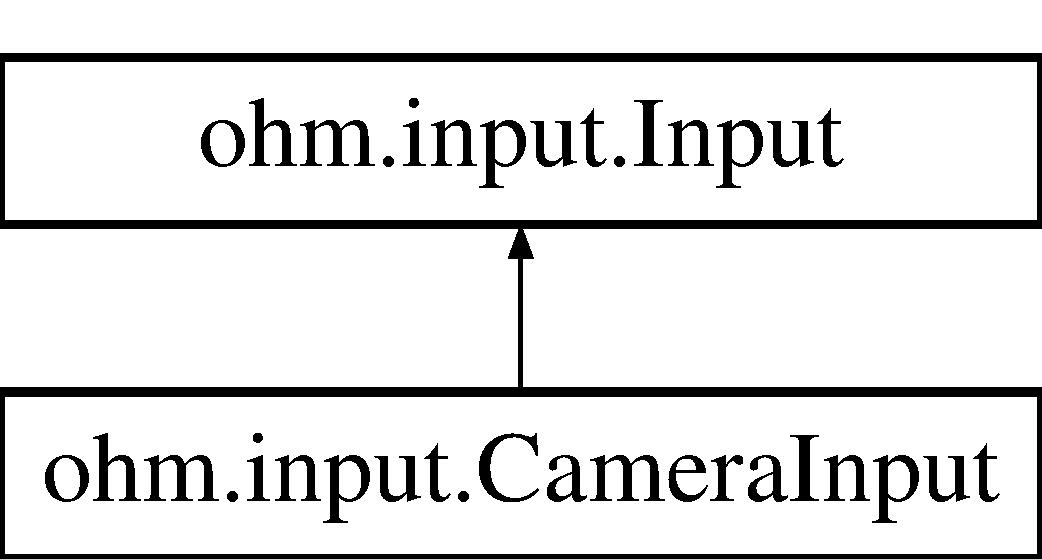
\includegraphics[height=2.000000cm]{classohm_1_1input_1_1_camera_input}
\end{center}
\end{figure}
\subsection*{Public Member Functions}
\begin{DoxyCompactItemize}
\item 
Image \hyperlink{classohm_1_1input_1_1_camera_input_a5d34760a889c9e574f8e3050bde679b6}{get\+Image} ()
\item 
Mat \hyperlink{classohm_1_1input_1_1_camera_input_ad237c282f6c3367ef857d12ebb079b38}{get\+R\+GB} ()
\item 
Mat \hyperlink{classohm_1_1input_1_1_camera_input_a1cee784ad09131e95ded21d07a42c8d4}{get\+L\+AB} ()
\end{DoxyCompactItemize}


\subsection{Detailed Description}
Class used to receive input from the camera on Desktop. 

\subsection{Member Function Documentation}
\hypertarget{classohm_1_1input_1_1_camera_input_a5d34760a889c9e574f8e3050bde679b6}{}\label{classohm_1_1input_1_1_camera_input_a5d34760a889c9e574f8e3050bde679b6} 
\index{ohm\+::input\+::\+Camera\+Input@{ohm\+::input\+::\+Camera\+Input}!get\+Image@{get\+Image}}
\index{get\+Image@{get\+Image}!ohm\+::input\+::\+Camera\+Input@{ohm\+::input\+::\+Camera\+Input}}
\subsubsection{\texorpdfstring{get\+Image()}{getImage()}}
{\footnotesize\ttfamily Image ohm.\+input.\+Camera\+Input.\+get\+Image (\begin{DoxyParamCaption}{ }\end{DoxyParamCaption})}

Used to retrieve a image representation of the input (used by Java\+FX). \begin{DoxyReturn}{Returns}
Image representation of input. 
\end{DoxyReturn}


Implements \hyperlink{interfaceohm_1_1input_1_1_input_aecea73d845b9c88e69294dadcd15e4fe}{ohm.\+input.\+Input}.

\hypertarget{classohm_1_1input_1_1_camera_input_a1cee784ad09131e95ded21d07a42c8d4}{}\label{classohm_1_1input_1_1_camera_input_a1cee784ad09131e95ded21d07a42c8d4} 
\index{ohm\+::input\+::\+Camera\+Input@{ohm\+::input\+::\+Camera\+Input}!get\+L\+AB@{get\+L\+AB}}
\index{get\+L\+AB@{get\+L\+AB}!ohm\+::input\+::\+Camera\+Input@{ohm\+::input\+::\+Camera\+Input}}
\subsubsection{\texorpdfstring{get\+L\+A\+B()}{getLAB()}}
{\footnotesize\ttfamily Mat ohm.\+input.\+Camera\+Input.\+get\+L\+AB (\begin{DoxyParamCaption}{ }\end{DoxyParamCaption})}

Used to retrieve a rgb matrix representation of the input (used by Opencv libraries). \begin{DoxyReturn}{Returns}
Matrix representation of input. 
\end{DoxyReturn}


Implements \hyperlink{interfaceohm_1_1input_1_1_input_a3264bf8e72c6442076453b5d356b6534}{ohm.\+input.\+Input}.

\hypertarget{classohm_1_1input_1_1_camera_input_ad237c282f6c3367ef857d12ebb079b38}{}\label{classohm_1_1input_1_1_camera_input_ad237c282f6c3367ef857d12ebb079b38} 
\index{ohm\+::input\+::\+Camera\+Input@{ohm\+::input\+::\+Camera\+Input}!get\+R\+GB@{get\+R\+GB}}
\index{get\+R\+GB@{get\+R\+GB}!ohm\+::input\+::\+Camera\+Input@{ohm\+::input\+::\+Camera\+Input}}
\subsubsection{\texorpdfstring{get\+R\+G\+B()}{getRGB()}}
{\footnotesize\ttfamily Mat ohm.\+input.\+Camera\+Input.\+get\+R\+GB (\begin{DoxyParamCaption}{ }\end{DoxyParamCaption})}

Used to retrieve a rgb matrix representation of the input (used by Opencv libraries). \begin{DoxyReturn}{Returns}
Matrix representation of input. 
\end{DoxyReturn}


Implements \hyperlink{interfaceohm_1_1input_1_1_input_ac9877f2cacdb85c06af084fd426495fd}{ohm.\+input.\+Input}.



The documentation for this class was generated from the following file\+:\begin{DoxyCompactItemize}
\item 
java/ohm/input/Camera\+Input.\+java\end{DoxyCompactItemize}

\hypertarget{classohm_1_1_helpers}{}\section{ohm.\+Helpers Class Reference}
\label{classohm_1_1_helpers}\index{ohm.\+Helpers@{ohm.\+Helpers}}
\subsection*{Static Public Member Functions}
\begin{DoxyCompactItemize}
\item 
\hypertarget{classohm_1_1_helpers_a1152a5e4b9a5206d82e72033dbb1ff19}{}\label{classohm_1_1_helpers_a1152a5e4b9a5206d82e72033dbb1ff19} 
static Image {\bfseries mat\+To\+Image} (Mat mat)
\end{DoxyCompactItemize}


\subsection{Detailed Description}
Module featuring static methods used by multiple other modules in order to perform common computations. Will be eliminated in final release. 

The documentation for this class was generated from the following file\+:\begin{DoxyCompactItemize}
\item 
java/ohm/Helpers.\+java\end{DoxyCompactItemize}

\hypertarget{classohm_1_1input_1_1_image_input}{}\section{ohm.\+input.\+Image\+Input Class Reference}
\label{classohm_1_1input_1_1_image_input}\index{ohm.\+input.\+Image\+Input@{ohm.\+input.\+Image\+Input}}


A source of input data, uses static images.  


Inheritance diagram for ohm.\+input.\+Image\+Input\+:\begin{figure}[H]
\begin{center}
\leavevmode
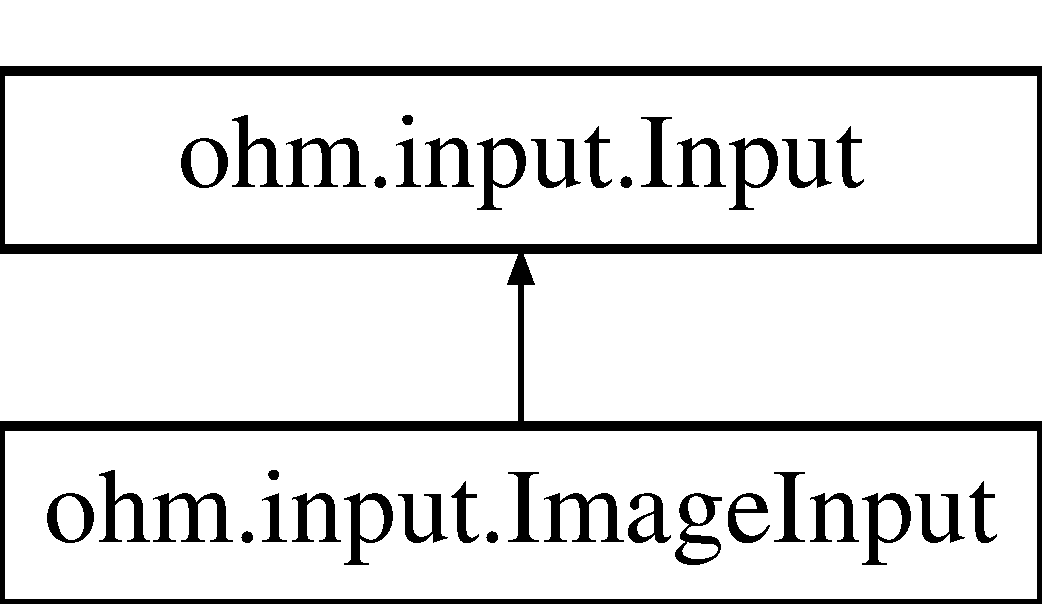
\includegraphics[height=2.000000cm]{classohm_1_1input_1_1_image_input}
\end{center}
\end{figure}
\subsection*{Public Member Functions}
\begin{DoxyCompactItemize}
\item 
\hyperlink{classohm_1_1input_1_1_image_input_af8fb2e251e80452993fd0400ae596628}{Image\+Input} ()
\item 
\hyperlink{classohm_1_1input_1_1_image_input_a3c9f1be5fc0574d2e2470c86fb1dbe90}{Image\+Input} (String name)
\item 
Mat \hyperlink{classohm_1_1input_1_1_image_input_aad0a18c0396fba14d5e1d74c08a592e6}{get\+R\+GB} ()
\item 
Image \hyperlink{classohm_1_1input_1_1_image_input_a68160a9bd9d395f7b2646e9b55388198}{get\+Image} ()
\item 
Mat \hyperlink{classohm_1_1input_1_1_image_input_a4f55591040c8129f3768948525d34863}{get\+L\+AB} ()
\end{DoxyCompactItemize}


\subsection{Detailed Description}
A source of input data, uses static images. 

\begin{DoxyAuthor}{Author}
Jonathan Brown 
\end{DoxyAuthor}


\subsection{Constructor \& Destructor Documentation}
\hypertarget{classohm_1_1input_1_1_image_input_af8fb2e251e80452993fd0400ae596628}{}\label{classohm_1_1input_1_1_image_input_af8fb2e251e80452993fd0400ae596628} 
\index{ohm\+::input\+::\+Image\+Input@{ohm\+::input\+::\+Image\+Input}!Image\+Input@{Image\+Input}}
\index{Image\+Input@{Image\+Input}!ohm\+::input\+::\+Image\+Input@{ohm\+::input\+::\+Image\+Input}}
\subsubsection{\texorpdfstring{Image\+Input()}{ImageInput()}\hspace{0.1cm}{\footnotesize\ttfamily [1/2]}}
{\footnotesize\ttfamily ohm.\+input.\+Image\+Input.\+Image\+Input (\begin{DoxyParamCaption}{ }\end{DoxyParamCaption})}

Default constructor creates an instance using a default image. \hypertarget{classohm_1_1input_1_1_image_input_a3c9f1be5fc0574d2e2470c86fb1dbe90}{}\label{classohm_1_1input_1_1_image_input_a3c9f1be5fc0574d2e2470c86fb1dbe90} 
\index{ohm\+::input\+::\+Image\+Input@{ohm\+::input\+::\+Image\+Input}!Image\+Input@{Image\+Input}}
\index{Image\+Input@{Image\+Input}!ohm\+::input\+::\+Image\+Input@{ohm\+::input\+::\+Image\+Input}}
\subsubsection{\texorpdfstring{Image\+Input()}{ImageInput()}\hspace{0.1cm}{\footnotesize\ttfamily [2/2]}}
{\footnotesize\ttfamily ohm.\+input.\+Image\+Input.\+Image\+Input (\begin{DoxyParamCaption}\item[{String}]{name }\end{DoxyParamCaption})}

Constructor featuring a name parameter. 
\begin{DoxyParams}{Parameters}
{\em name} & The name of the input image. Do not include an extension. \\
\hline
\end{DoxyParams}


\subsection{Member Function Documentation}
\hypertarget{classohm_1_1input_1_1_image_input_a68160a9bd9d395f7b2646e9b55388198}{}\label{classohm_1_1input_1_1_image_input_a68160a9bd9d395f7b2646e9b55388198} 
\index{ohm\+::input\+::\+Image\+Input@{ohm\+::input\+::\+Image\+Input}!get\+Image@{get\+Image}}
\index{get\+Image@{get\+Image}!ohm\+::input\+::\+Image\+Input@{ohm\+::input\+::\+Image\+Input}}
\subsubsection{\texorpdfstring{get\+Image()}{getImage()}}
{\footnotesize\ttfamily Image ohm.\+input.\+Image\+Input.\+get\+Image (\begin{DoxyParamCaption}{ }\end{DoxyParamCaption})}

Used to retrieve a image representation of the input (used by Java\+FX). \begin{DoxyReturn}{Returns}
Image representation of input. 
\end{DoxyReturn}


Implements \hyperlink{interfaceohm_1_1input_1_1_input_aecea73d845b9c88e69294dadcd15e4fe}{ohm.\+input.\+Input}.

\hypertarget{classohm_1_1input_1_1_image_input_a4f55591040c8129f3768948525d34863}{}\label{classohm_1_1input_1_1_image_input_a4f55591040c8129f3768948525d34863} 
\index{ohm\+::input\+::\+Image\+Input@{ohm\+::input\+::\+Image\+Input}!get\+L\+AB@{get\+L\+AB}}
\index{get\+L\+AB@{get\+L\+AB}!ohm\+::input\+::\+Image\+Input@{ohm\+::input\+::\+Image\+Input}}
\subsubsection{\texorpdfstring{get\+L\+A\+B()}{getLAB()}}
{\footnotesize\ttfamily Mat ohm.\+input.\+Image\+Input.\+get\+L\+AB (\begin{DoxyParamCaption}{ }\end{DoxyParamCaption})}

Used to retrieve a rgb matrix representation of the input (used by Opencv libraries). \begin{DoxyReturn}{Returns}
Matrix representation of input. 
\end{DoxyReturn}


Implements \hyperlink{interfaceohm_1_1input_1_1_input_a3264bf8e72c6442076453b5d356b6534}{ohm.\+input.\+Input}.

\hypertarget{classohm_1_1input_1_1_image_input_aad0a18c0396fba14d5e1d74c08a592e6}{}\label{classohm_1_1input_1_1_image_input_aad0a18c0396fba14d5e1d74c08a592e6} 
\index{ohm\+::input\+::\+Image\+Input@{ohm\+::input\+::\+Image\+Input}!get\+R\+GB@{get\+R\+GB}}
\index{get\+R\+GB@{get\+R\+GB}!ohm\+::input\+::\+Image\+Input@{ohm\+::input\+::\+Image\+Input}}
\subsubsection{\texorpdfstring{get\+R\+G\+B()}{getRGB()}}
{\footnotesize\ttfamily Mat ohm.\+input.\+Image\+Input.\+get\+R\+GB (\begin{DoxyParamCaption}{ }\end{DoxyParamCaption})}

Method returns a Open\+CV Matrix of the loaded image. \begin{DoxyReturn}{Returns}
Open\+CV Matrix representation of the image. 
\end{DoxyReturn}


Implements \hyperlink{interfaceohm_1_1input_1_1_input_ac9877f2cacdb85c06af084fd426495fd}{ohm.\+input.\+Input}.



The documentation for this class was generated from the following file\+:\begin{DoxyCompactItemize}
\item 
java/ohm/input/Image\+Input.\+java\end{DoxyCompactItemize}

\hypertarget{interfaceohm_1_1input_1_1_input}{}\section{ohm.\+input.\+Input Interface Reference}
\label{interfaceohm_1_1input_1_1_input}\index{ohm.\+input.\+Input@{ohm.\+input.\+Input}}
Inheritance diagram for ohm.\+input.\+Input\+:\begin{figure}[H]
\begin{center}
\leavevmode
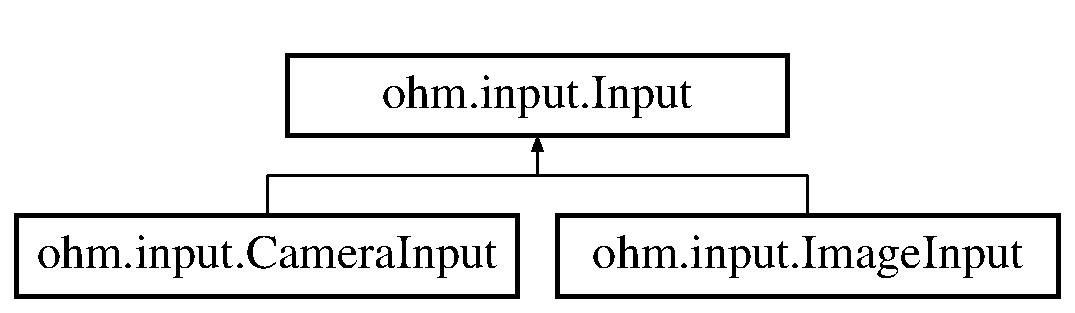
\includegraphics[height=2.000000cm]{interfaceohm_1_1input_1_1_input}
\end{center}
\end{figure}
\subsection*{Public Member Functions}
\begin{DoxyCompactItemize}
\item 
Mat \hyperlink{interfaceohm_1_1input_1_1_input_ac9877f2cacdb85c06af084fd426495fd}{get\+R\+GB} ()
\item 
Image \hyperlink{interfaceohm_1_1input_1_1_input_aecea73d845b9c88e69294dadcd15e4fe}{get\+Image} ()
\item 
Mat \hyperlink{interfaceohm_1_1input_1_1_input_a3264bf8e72c6442076453b5d356b6534}{get\+L\+AB} ()
\end{DoxyCompactItemize}


\subsection{Detailed Description}
\begin{DoxyAuthor}{Author}
Jonathan Brown 
\end{DoxyAuthor}


\subsection{Member Function Documentation}
\hypertarget{interfaceohm_1_1input_1_1_input_aecea73d845b9c88e69294dadcd15e4fe}{}\label{interfaceohm_1_1input_1_1_input_aecea73d845b9c88e69294dadcd15e4fe} 
\index{ohm\+::input\+::\+Input@{ohm\+::input\+::\+Input}!get\+Image@{get\+Image}}
\index{get\+Image@{get\+Image}!ohm\+::input\+::\+Input@{ohm\+::input\+::\+Input}}
\subsubsection{\texorpdfstring{get\+Image()}{getImage()}}
{\footnotesize\ttfamily Image ohm.\+input.\+Input.\+get\+Image (\begin{DoxyParamCaption}{ }\end{DoxyParamCaption})}

Used to retrieve a image representation of the input (used by Java\+FX). \begin{DoxyReturn}{Returns}
Image representation of input. 
\end{DoxyReturn}


Implemented in \hyperlink{classohm_1_1input_1_1_camera_input_a5d34760a889c9e574f8e3050bde679b6}{ohm.\+input.\+Camera\+Input}, and \hyperlink{classohm_1_1input_1_1_image_input_a68160a9bd9d395f7b2646e9b55388198}{ohm.\+input.\+Image\+Input}.

\hypertarget{interfaceohm_1_1input_1_1_input_a3264bf8e72c6442076453b5d356b6534}{}\label{interfaceohm_1_1input_1_1_input_a3264bf8e72c6442076453b5d356b6534} 
\index{ohm\+::input\+::\+Input@{ohm\+::input\+::\+Input}!get\+L\+AB@{get\+L\+AB}}
\index{get\+L\+AB@{get\+L\+AB}!ohm\+::input\+::\+Input@{ohm\+::input\+::\+Input}}
\subsubsection{\texorpdfstring{get\+L\+A\+B()}{getLAB()}}
{\footnotesize\ttfamily Mat ohm.\+input.\+Input.\+get\+L\+AB (\begin{DoxyParamCaption}{ }\end{DoxyParamCaption})}

Used to retrieve a rgb matrix representation of the input (used by Opencv libraries). \begin{DoxyReturn}{Returns}
Matrix representation of input. 
\end{DoxyReturn}


Implemented in \hyperlink{classohm_1_1input_1_1_camera_input_a1cee784ad09131e95ded21d07a42c8d4}{ohm.\+input.\+Camera\+Input}, and \hyperlink{classohm_1_1input_1_1_image_input_a4f55591040c8129f3768948525d34863}{ohm.\+input.\+Image\+Input}.

\hypertarget{interfaceohm_1_1input_1_1_input_ac9877f2cacdb85c06af084fd426495fd}{}\label{interfaceohm_1_1input_1_1_input_ac9877f2cacdb85c06af084fd426495fd} 
\index{ohm\+::input\+::\+Input@{ohm\+::input\+::\+Input}!get\+R\+GB@{get\+R\+GB}}
\index{get\+R\+GB@{get\+R\+GB}!ohm\+::input\+::\+Input@{ohm\+::input\+::\+Input}}
\subsubsection{\texorpdfstring{get\+R\+G\+B()}{getRGB()}}
{\footnotesize\ttfamily Mat ohm.\+input.\+Input.\+get\+R\+GB (\begin{DoxyParamCaption}{ }\end{DoxyParamCaption})}

Used to retrieve a rgb matrix representation of the input (used by Opencv libraries). \begin{DoxyReturn}{Returns}
Matrix representation of input. 
\end{DoxyReturn}


Implemented in \hyperlink{classohm_1_1input_1_1_camera_input_ad237c282f6c3367ef857d12ebb079b38}{ohm.\+input.\+Camera\+Input}, and \hyperlink{classohm_1_1input_1_1_image_input_aad0a18c0396fba14d5e1d74c08a592e6}{ohm.\+input.\+Image\+Input}.



The documentation for this interface was generated from the following file\+:\begin{DoxyCompactItemize}
\item 
java/ohm/input/Input.\+java\end{DoxyCompactItemize}

\hypertarget{classohm_1_1userinterface_1_1_live_image_view}{}\section{ohm.\+userinterface.\+Live\+Image\+View Class Reference}
\label{classohm_1_1userinterface_1_1_live_image_view}\index{ohm.\+userinterface.\+Live\+Image\+View@{ohm.\+userinterface.\+Live\+Image\+View}}


The \hyperlink{classohm_1_1userinterface_1_1_live_image_view}{Live\+Image\+View} is an Image\+View that periodically calls a Renderer to produce a new image that the Image\+View then displays. This is useful to create images from real time updating images/data.  


Inheritance diagram for ohm.\+userinterface.\+Live\+Image\+View\+:\begin{figure}[H]
\begin{center}
\leavevmode
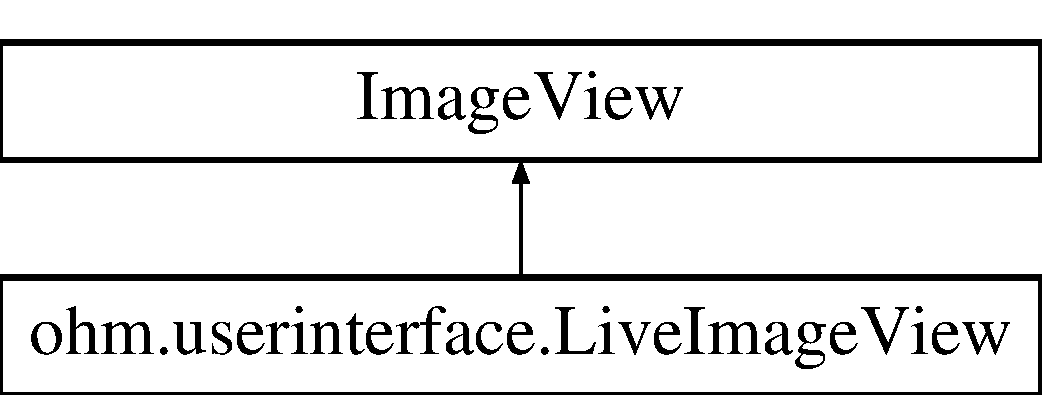
\includegraphics[height=2.000000cm]{classohm_1_1userinterface_1_1_live_image_view}
\end{center}
\end{figure}
\subsection*{Classes}
\begin{DoxyCompactItemize}
\item 
interface {\bfseries Renderer}
\end{DoxyCompactItemize}
\subsection*{Public Member Functions}
\begin{DoxyCompactItemize}
\item 
\hypertarget{classohm_1_1userinterface_1_1_live_image_view_adb27a4d64d1d6ad4b5141fbc021f493d}{}\label{classohm_1_1userinterface_1_1_live_image_view_adb27a4d64d1d6ad4b5141fbc021f493d} 
void {\bfseries set\+Frame\+Rate} (int frame\+Rate)
\item 
\hypertarget{classohm_1_1userinterface_1_1_live_image_view_adc84c60fead29aa42106096efcb1912c}{}\label{classohm_1_1userinterface_1_1_live_image_view_adc84c60fead29aa42106096efcb1912c} 
void {\bfseries set\+Renderer} (Renderer new\+Renderer)
\end{DoxyCompactItemize}


\subsection{Detailed Description}
The \hyperlink{classohm_1_1userinterface_1_1_live_image_view}{Live\+Image\+View} is an Image\+View that periodically calls a Renderer to produce a new image that the Image\+View then displays. This is useful to create images from real time updating images/data. 

The documentation for this class was generated from the following file\+:\begin{DoxyCompactItemize}
\item 
java/ohm/userinterface/Live\+Image\+View.\+java\end{DoxyCompactItemize}

\hypertarget{classohm_1_1_ohm}{}\section{ohm.\+Ohm Class Reference}
\label{classohm_1_1_ohm}\index{ohm.\+Ohm@{ohm.\+Ohm}}
Inheritance diagram for ohm.\+Ohm\+:\begin{figure}[H]
\begin{center}
\leavevmode
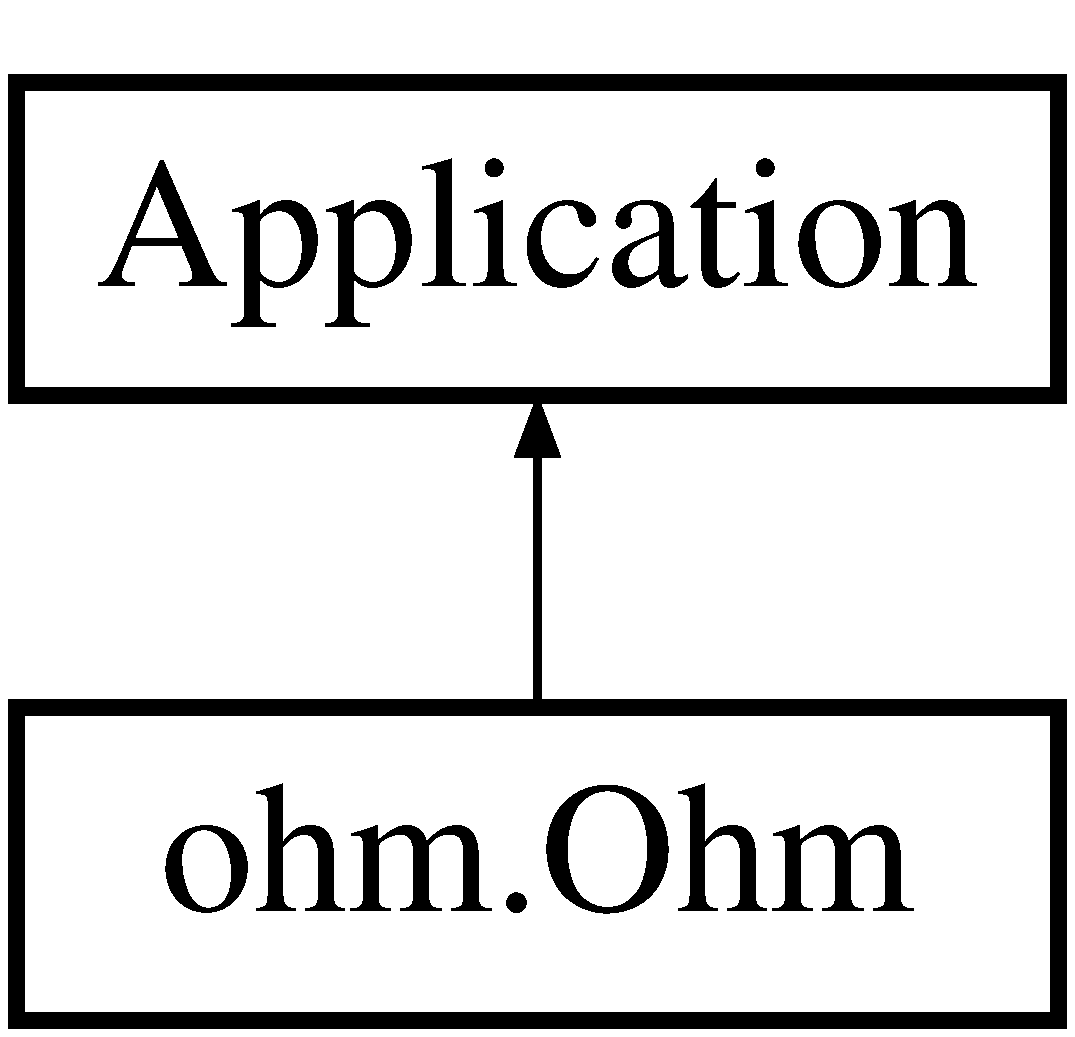
\includegraphics[height=2.000000cm]{classohm_1_1_ohm}
\end{center}
\end{figure}
\subsection*{Public Member Functions}
\begin{DoxyCompactItemize}
\item 
\hypertarget{classohm_1_1_ohm_aa571bf3c8c1419af5e4b875293ac6123}{}\label{classohm_1_1_ohm_aa571bf3c8c1419af5e4b875293ac6123} 
void {\bfseries start} (Stage primary\+Stage)  throws Exception
\end{DoxyCompactItemize}
\subsection*{Static Public Member Functions}
\begin{DoxyCompactItemize}
\item 
\hypertarget{classohm_1_1_ohm_a0ac90b2134f0974b8dd2d657cdcf99a2}{}\label{classohm_1_1_ohm_a0ac90b2134f0974b8dd2d657cdcf99a2} 
static void {\bfseries main} (String\mbox{[}$\,$\mbox{]} args)  throws Exception
\end{DoxyCompactItemize}


The documentation for this class was generated from the following file\+:\begin{DoxyCompactItemize}
\item 
java/ohm/Ohm.\+java\end{DoxyCompactItemize}

\hypertarget{classohm_1_1userinterface_1_1_ohm_view_controller}{}\section{ohm.\+userinterface.\+Ohm\+View\+Controller Class Reference}
\label{classohm_1_1userinterface_1_1_ohm_view_controller}\index{ohm.\+userinterface.\+Ohm\+View\+Controller@{ohm.\+userinterface.\+Ohm\+View\+Controller}}


Coordinates the algorithms present in the model with user input through the view.  


Inheritance diagram for ohm.\+userinterface.\+Ohm\+View\+Controller\+:\begin{figure}[H]
\begin{center}
\leavevmode
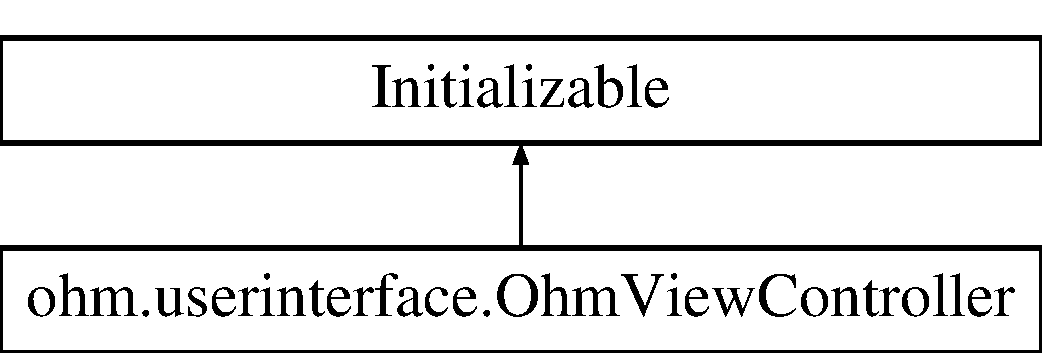
\includegraphics[height=2.000000cm]{classohm_1_1userinterface_1_1_ohm_view_controller}
\end{center}
\end{figure}
\subsection*{Public Member Functions}
\begin{DoxyCompactItemize}
\item 
void \hyperlink{classohm_1_1userinterface_1_1_ohm_view_controller_aa1653060f9f810ea5cd6a0f917b02521}{initialize} (U\+RL url, Resource\+Bundle rb)
\item 
\hypertarget{classohm_1_1userinterface_1_1_ohm_view_controller_ab5c13417b6bd773de779c08757988824}{}\label{classohm_1_1userinterface_1_1_ohm_view_controller_ab5c13417b6bd773de779c08757988824} 
void {\bfseries button\+Clicked} (Action\+Event action\+Event)
\end{DoxyCompactItemize}
\subsection*{Public Attributes}
\begin{DoxyCompactItemize}
\item 
\hypertarget{classohm_1_1userinterface_1_1_ohm_view_controller_a3d5fcbb87065c909362db6e2b08ac990}{}\label{classohm_1_1userinterface_1_1_ohm_view_controller_a3d5fcbb87065c909362db6e2b08ac990} 
Button {\bfseries start\+Camera\+Button}
\end{DoxyCompactItemize}


\subsection{Detailed Description}
Coordinates the algorithms present in the model with user input through the view. 

\subsection{Member Function Documentation}
\hypertarget{classohm_1_1userinterface_1_1_ohm_view_controller_aa1653060f9f810ea5cd6a0f917b02521}{}\label{classohm_1_1userinterface_1_1_ohm_view_controller_aa1653060f9f810ea5cd6a0f917b02521} 
\index{ohm\+::userinterface\+::\+Ohm\+View\+Controller@{ohm\+::userinterface\+::\+Ohm\+View\+Controller}!initialize@{initialize}}
\index{initialize@{initialize}!ohm\+::userinterface\+::\+Ohm\+View\+Controller@{ohm\+::userinterface\+::\+Ohm\+View\+Controller}}
\subsubsection{\texorpdfstring{initialize()}{initialize()}}
{\footnotesize\ttfamily void ohm.\+userinterface.\+Ohm\+View\+Controller.\+initialize (\begin{DoxyParamCaption}\item[{U\+RL}]{url,  }\item[{Resource\+Bundle}]{rb }\end{DoxyParamCaption})}

Method used to \char`\"{}glue\char`\"{} together the front and back end of the application. 

The documentation for this class was generated from the following file\+:\begin{DoxyCompactItemize}
\item 
java/ohm/userinterface/Ohm\+View\+Controller.\+java\end{DoxyCompactItemize}

\hypertarget{classohm_1_1userinterface_1_1_resistor_axis_picker_view}{}\section{ohm.\+userinterface.\+Resistor\+Axis\+Picker\+View Class Reference}
\label{classohm_1_1userinterface_1_1_resistor_axis_picker_view}\index{ohm.\+userinterface.\+Resistor\+Axis\+Picker\+View@{ohm.\+userinterface.\+Resistor\+Axis\+Picker\+View}}


This class displays an opencv Mat as an image and allows the user to pick two endpoints of a line. Once two valid points, a listener is called.  


Inheritance diagram for ohm.\+userinterface.\+Resistor\+Axis\+Picker\+View\+:\begin{figure}[H]
\begin{center}
\leavevmode
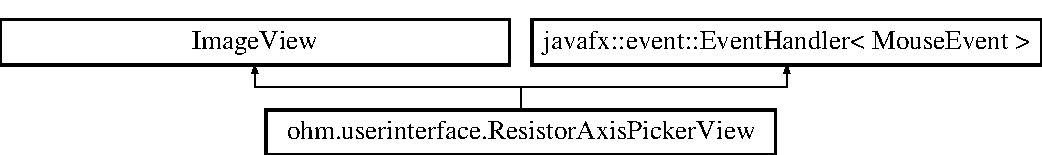
\includegraphics[height=2.000000cm]{classohm_1_1userinterface_1_1_resistor_axis_picker_view}
\end{center}
\end{figure}
\subsection*{Classes}
\begin{DoxyCompactItemize}
\item 
interface {\bfseries Listener}
\end{DoxyCompactItemize}
\subsection*{Public Member Functions}
\begin{DoxyCompactItemize}
\item 
\hypertarget{classohm_1_1userinterface_1_1_resistor_axis_picker_view_a18f03b2e9fbfd47ce86d525dbd9aadd7}{}\label{classohm_1_1userinterface_1_1_resistor_axis_picker_view_a18f03b2e9fbfd47ce86d525dbd9aadd7} 
void {\bfseries handle} (Mouse\+Event event)
\item 
void \hyperlink{classohm_1_1userinterface_1_1_resistor_axis_picker_view_aca0066d9015235e9379505a8e89543b1}{set\+Image} (Mat new\+Image)
\item 
void \hyperlink{classohm_1_1userinterface_1_1_resistor_axis_picker_view_a78a2696e3a51570963bbf23870bee204}{set\+Listener} (Listener listener)
\end{DoxyCompactItemize}
\subsection*{Static Public Member Functions}
\begin{DoxyCompactItemize}
\item 
\hypertarget{classohm_1_1userinterface_1_1_resistor_axis_picker_view_a09ec66453bd16e8f693d7bddc16aed9e}{}\label{classohm_1_1userinterface_1_1_resistor_axis_picker_view_a09ec66453bd16e8f693d7bddc16aed9e} 
static double {\bfseries dist} (Point p1, Point p2)
\end{DoxyCompactItemize}


\subsection{Detailed Description}
This class displays an opencv Mat as an image and allows the user to pick two endpoints of a line. Once two valid points, a listener is called. 

\subsection{Member Function Documentation}
\hypertarget{classohm_1_1userinterface_1_1_resistor_axis_picker_view_aca0066d9015235e9379505a8e89543b1}{}\label{classohm_1_1userinterface_1_1_resistor_axis_picker_view_aca0066d9015235e9379505a8e89543b1} 
\index{ohm\+::userinterface\+::\+Resistor\+Axis\+Picker\+View@{ohm\+::userinterface\+::\+Resistor\+Axis\+Picker\+View}!set\+Image@{set\+Image}}
\index{set\+Image@{set\+Image}!ohm\+::userinterface\+::\+Resistor\+Axis\+Picker\+View@{ohm\+::userinterface\+::\+Resistor\+Axis\+Picker\+View}}
\subsubsection{\texorpdfstring{set\+Image()}{setImage()}}
{\footnotesize\ttfamily void ohm.\+userinterface.\+Resistor\+Axis\+Picker\+View.\+set\+Image (\begin{DoxyParamCaption}\item[{Mat}]{new\+Image }\end{DoxyParamCaption})}

Set the matrix to display 
\begin{DoxyParams}{Parameters}
{\em new\+Image} & Image to be set as the image to be displayed in the UI \\
\hline
\end{DoxyParams}
\hypertarget{classohm_1_1userinterface_1_1_resistor_axis_picker_view_a78a2696e3a51570963bbf23870bee204}{}\label{classohm_1_1userinterface_1_1_resistor_axis_picker_view_a78a2696e3a51570963bbf23870bee204} 
\index{ohm\+::userinterface\+::\+Resistor\+Axis\+Picker\+View@{ohm\+::userinterface\+::\+Resistor\+Axis\+Picker\+View}!set\+Listener@{set\+Listener}}
\index{set\+Listener@{set\+Listener}!ohm\+::userinterface\+::\+Resistor\+Axis\+Picker\+View@{ohm\+::userinterface\+::\+Resistor\+Axis\+Picker\+View}}
\subsubsection{\texorpdfstring{set\+Listener()}{setListener()}}
{\footnotesize\ttfamily void ohm.\+userinterface.\+Resistor\+Axis\+Picker\+View.\+set\+Listener (\begin{DoxyParamCaption}\item[{Listener}]{listener }\end{DoxyParamCaption})}

Assign a line listener to be updated when new points are selected 
\begin{DoxyParams}{Parameters}
{\em listener} & Object that triggers responds to a mouse click inside the view. \\
\hline
\end{DoxyParams}


The documentation for this class was generated from the following file\+:\begin{DoxyCompactItemize}
\item 
java/ohm/userinterface/Resistor\+Axis\+Picker\+View.\+java\end{DoxyCompactItemize}

\hypertarget{enumohm_1_1valueidentification_1_1_resistor_colour}{}\section{ohm.\+valueidentification.\+Resistor\+Colour Enum Reference}
\label{enumohm_1_1valueidentification_1_1_resistor_colour}\index{ohm.\+valueidentification.\+Resistor\+Colour@{ohm.\+valueidentification.\+Resistor\+Colour}}


Enum containing all of the possible colours that a resistor can take on. Also features member functions used to map the colours of bands to values used in the calculation process.  


\subsection*{Public Member Functions}
\begin{DoxyCompactItemize}
\item 
\hyperlink{enumohm_1_1valueidentification_1_1_resistor_colour_a5828a5bf9478083a393751137153d659}{Resistor\+Colour} (int v)
\end{DoxyCompactItemize}
\subsection*{Static Public Member Functions}
\begin{DoxyCompactItemize}
\item 
\hyperlink{enumohm_1_1valueidentification_1_1_resistor_colour_ada1c80467eac208be473beadf83f968f}{\mbox{[}static initializer\mbox{]}}
\item 
static void \hyperlink{enumohm_1_1valueidentification_1_1_resistor_colour_a9c01747715aac184cde55a4161ccfe44}{rgb2lab} (float R, float G, float B, float\mbox{[}$\,$\mbox{]} lab)
\item 
\hypertarget{enumohm_1_1valueidentification_1_1_resistor_colour_a64c975f538d0040ef0ec5b2376a6ace7}{}\label{enumohm_1_1valueidentification_1_1_resistor_colour_a64c975f538d0040ef0ec5b2376a6ace7} 
static int {\bfseries fit} (float r, float g, float b)
\item 
static int \hyperlink{enumohm_1_1valueidentification_1_1_resistor_colour_a054bf549f7693e59f813f83d7b93148b}{fit} (int r, int g, int b, int color\+Space)
\item 
static int \hyperlink{enumohm_1_1valueidentification_1_1_resistor_colour_a04dc2256f1c7b0ffbe9edd9d85dd9fc6}{fit} (double r, double g, double b, int color\+Space)
\end{DoxyCompactItemize}
\subsection*{Public Attributes}
\begin{DoxyCompactItemize}
\item 
\hypertarget{enumohm_1_1valueidentification_1_1_resistor_colour_a3f4296ddc45bf34f4e8106d8446ed886}{}\label{enumohm_1_1valueidentification_1_1_resistor_colour_a3f4296ddc45bf34f4e8106d8446ed886} 
{\bfseries B\+L\+A\+CK} =(0)
\item 
\hypertarget{enumohm_1_1valueidentification_1_1_resistor_colour_a4a8266a81a9f5f41f26e36cfdf903023}{}\label{enumohm_1_1valueidentification_1_1_resistor_colour_a4a8266a81a9f5f41f26e36cfdf903023} 
{\bfseries B\+R\+O\+WN} =(1)
\item 
\hypertarget{enumohm_1_1valueidentification_1_1_resistor_colour_abc23efde99204e31b73335b4537eade8}{}\label{enumohm_1_1valueidentification_1_1_resistor_colour_abc23efde99204e31b73335b4537eade8} 
{\bfseries R\+ED} =(2)
\item 
\hypertarget{enumohm_1_1valueidentification_1_1_resistor_colour_a01f360dd4c0c3927003b44596d1b21a9}{}\label{enumohm_1_1valueidentification_1_1_resistor_colour_a01f360dd4c0c3927003b44596d1b21a9} 
{\bfseries O\+R\+A\+N\+GE} =(3)
\item 
\hypertarget{enumohm_1_1valueidentification_1_1_resistor_colour_af7c6e68f5594ba0fc1c762059ae108af}{}\label{enumohm_1_1valueidentification_1_1_resistor_colour_af7c6e68f5594ba0fc1c762059ae108af} 
{\bfseries Y\+E\+L\+L\+OW} =(4)
\item 
\hypertarget{enumohm_1_1valueidentification_1_1_resistor_colour_a1161918898b8bc9ef3346208cc7b7571}{}\label{enumohm_1_1valueidentification_1_1_resistor_colour_a1161918898b8bc9ef3346208cc7b7571} 
{\bfseries G\+R\+E\+EN} =(5)
\item 
\hypertarget{enumohm_1_1valueidentification_1_1_resistor_colour_a74020b01a380db115093b40d32e6270c}{}\label{enumohm_1_1valueidentification_1_1_resistor_colour_a74020b01a380db115093b40d32e6270c} 
{\bfseries B\+L\+UE} =(6)
\item 
\hypertarget{enumohm_1_1valueidentification_1_1_resistor_colour_a6dfde419d67bfdf6106e0b120c28aa00}{}\label{enumohm_1_1valueidentification_1_1_resistor_colour_a6dfde419d67bfdf6106e0b120c28aa00} 
{\bfseries V\+I\+O\+L\+ET} =(7)
\item 
\hypertarget{enumohm_1_1valueidentification_1_1_resistor_colour_a57fd5d586f515193a82346ac5e525817}{}\label{enumohm_1_1valueidentification_1_1_resistor_colour_a57fd5d586f515193a82346ac5e525817} 
{\bfseries G\+R\+EY} =(8)
\item 
\hypertarget{enumohm_1_1valueidentification_1_1_resistor_colour_a0f173e15f1e62f7f1c4e80ba5991dd87}{}\label{enumohm_1_1valueidentification_1_1_resistor_colour_a0f173e15f1e62f7f1c4e80ba5991dd87} 
{\bfseries W\+H\+I\+TE} =(9)
\item 
\hypertarget{enumohm_1_1valueidentification_1_1_resistor_colour_a0094d82b0ce5aa8e11a1dd86d370ea09}{}\label{enumohm_1_1valueidentification_1_1_resistor_colour_a0094d82b0ce5aa8e11a1dd86d370ea09} 
{\bfseries G\+O\+LD} =(11)
\item 
\hypertarget{enumohm_1_1valueidentification_1_1_resistor_colour_a14ef1a48b49d8038d07d2c067023cb49}{}\label{enumohm_1_1valueidentification_1_1_resistor_colour_a14ef1a48b49d8038d07d2c067023cb49} 
{\bfseries B\+A\+SE} =(10)
\item 
\hypertarget{enumohm_1_1valueidentification_1_1_resistor_colour_a7ce9ef407d138453603a0886d22cbf8d}{}\label{enumohm_1_1valueidentification_1_1_resistor_colour_a7ce9ef407d138453603a0886d22cbf8d} 
int {\bfseries value}
\end{DoxyCompactItemize}
\subsection*{Static Public Attributes}
\begin{DoxyCompactItemize}
\item 
\hypertarget{enumohm_1_1valueidentification_1_1_resistor_colour_a6cbfec1e6406faa4415abb349178fd53}{}\label{enumohm_1_1valueidentification_1_1_resistor_colour_a6cbfec1e6406faa4415abb349178fd53} 
static K\+Nearest {\bfseries K\+NN}
\end{DoxyCompactItemize}


\subsection{Detailed Description}
Enum containing all of the possible colours that a resistor can take on. Also features member functions used to map the colours of bands to values used in the calculation process. 

\subsection{Constructor \& Destructor Documentation}
\hypertarget{enumohm_1_1valueidentification_1_1_resistor_colour_a5828a5bf9478083a393751137153d659}{}\label{enumohm_1_1valueidentification_1_1_resistor_colour_a5828a5bf9478083a393751137153d659} 
\index{ohm\+::valueidentification\+::\+Resistor\+Colour@{ohm\+::valueidentification\+::\+Resistor\+Colour}!Resistor\+Colour@{Resistor\+Colour}}
\index{Resistor\+Colour@{Resistor\+Colour}!ohm\+::valueidentification\+::\+Resistor\+Colour@{ohm\+::valueidentification\+::\+Resistor\+Colour}}
\subsubsection{\texorpdfstring{Resistor\+Colour()}{ResistorColour()}}
{\footnotesize\ttfamily ohm.\+valueidentification.\+Resistor\+Colour.\+Resistor\+Colour (\begin{DoxyParamCaption}\item[{int}]{v }\end{DoxyParamCaption})}


\begin{DoxyItemize}
\item 
\begin{DoxyParams}{Parameters}
{\em v} & The number represented by the colour in the calculation of the resistor\textquotesingle{}s ohmage. \\
\hline
\end{DoxyParams}

\end{DoxyItemize}

\subsection{Member Function Documentation}
\hypertarget{enumohm_1_1valueidentification_1_1_resistor_colour_ada1c80467eac208be473beadf83f968f}{}\label{enumohm_1_1valueidentification_1_1_resistor_colour_ada1c80467eac208be473beadf83f968f} 
\index{ohm\+::valueidentification\+::\+Resistor\+Colour@{ohm\+::valueidentification\+::\+Resistor\+Colour}!\mbox{[}static initializer\mbox{]}@{[static initializer]}}
\index{\mbox{[}static initializer\mbox{]}@{[static initializer]}!ohm\+::valueidentification\+::\+Resistor\+Colour@{ohm\+::valueidentification\+::\+Resistor\+Colour}}
\subsubsection{\texorpdfstring{[static initializer]()}{[static initializer]()}}
{\footnotesize\ttfamily ohm.\+valueidentification.\+Resistor\+Colour.\mbox{[}static initializer\mbox{]} (\begin{DoxyParamCaption}{ }\end{DoxyParamCaption})\hspace{0.3cm}{\ttfamily [static]}}

Creates and trains the K\+NN classifier. Based on the training set stored in train.\+csv. \hypertarget{enumohm_1_1valueidentification_1_1_resistor_colour_a054bf549f7693e59f813f83d7b93148b}{}\label{enumohm_1_1valueidentification_1_1_resistor_colour_a054bf549f7693e59f813f83d7b93148b} 
\index{ohm\+::valueidentification\+::\+Resistor\+Colour@{ohm\+::valueidentification\+::\+Resistor\+Colour}!fit@{fit}}
\index{fit@{fit}!ohm\+::valueidentification\+::\+Resistor\+Colour@{ohm\+::valueidentification\+::\+Resistor\+Colour}}
\subsubsection{\texorpdfstring{fit()}{fit()}\hspace{0.1cm}{\footnotesize\ttfamily [1/2]}}
{\footnotesize\ttfamily static int ohm.\+valueidentification.\+Resistor\+Colour.\+fit (\begin{DoxyParamCaption}\item[{int}]{r,  }\item[{int}]{g,  }\item[{int}]{b,  }\item[{int}]{color\+Space }\end{DoxyParamCaption})\hspace{0.3cm}{\ttfamily [static]}}

Function takes in a sampled colour from the images and attempts to fit\+Old it to the closest known colour a resistor can possess. 
\begin{DoxyParams}{Parameters}
{\em r} & The red colour value of the colour to be fit\+Old. \\
\hline
{\em g} & The green colour value of the colour to be fit\+Old. \\
\hline
{\em b} & The blue colour value of the colour to be fit\+Old. \\
\hline
\end{DoxyParams}
\begin{DoxyReturn}{Returns}
The known colour that best represents the sampled colour. 
\end{DoxyReturn}
\hypertarget{enumohm_1_1valueidentification_1_1_resistor_colour_a04dc2256f1c7b0ffbe9edd9d85dd9fc6}{}\label{enumohm_1_1valueidentification_1_1_resistor_colour_a04dc2256f1c7b0ffbe9edd9d85dd9fc6} 
\index{ohm\+::valueidentification\+::\+Resistor\+Colour@{ohm\+::valueidentification\+::\+Resistor\+Colour}!fit@{fit}}
\index{fit@{fit}!ohm\+::valueidentification\+::\+Resistor\+Colour@{ohm\+::valueidentification\+::\+Resistor\+Colour}}
\subsubsection{\texorpdfstring{fit()}{fit()}\hspace{0.1cm}{\footnotesize\ttfamily [2/2]}}
{\footnotesize\ttfamily static int ohm.\+valueidentification.\+Resistor\+Colour.\+fit (\begin{DoxyParamCaption}\item[{double}]{r,  }\item[{double}]{g,  }\item[{double}]{b,  }\item[{int}]{color\+Space }\end{DoxyParamCaption})\hspace{0.3cm}{\ttfamily [static]}}

Function takes in a sampled colour from the images and attempts to fit\+Old it to the closest known colour a resistor can possess. 
\begin{DoxyParams}{Parameters}
{\em r} & The red colour value of the colour to be fit\+Old. \\
\hline
{\em g} & The green colour value of the colour to be fit\+Old. \\
\hline
{\em b} & The blue colour value of the colour to be fit\+Old. \\
\hline
\end{DoxyParams}
\begin{DoxyReturn}{Returns}
The known colour that best represents the sampled colour. 
\end{DoxyReturn}
\hypertarget{enumohm_1_1valueidentification_1_1_resistor_colour_a9c01747715aac184cde55a4161ccfe44}{}\label{enumohm_1_1valueidentification_1_1_resistor_colour_a9c01747715aac184cde55a4161ccfe44} 
\index{ohm\+::valueidentification\+::\+Resistor\+Colour@{ohm\+::valueidentification\+::\+Resistor\+Colour}!rgb2lab@{rgb2lab}}
\index{rgb2lab@{rgb2lab}!ohm\+::valueidentification\+::\+Resistor\+Colour@{ohm\+::valueidentification\+::\+Resistor\+Colour}}
\subsubsection{\texorpdfstring{rgb2lab()}{rgb2lab()}}
{\footnotesize\ttfamily static void ohm.\+valueidentification.\+Resistor\+Colour.\+rgb2lab (\begin{DoxyParamCaption}\item[{float}]{R,  }\item[{float}]{G,  }\item[{float}]{B,  }\item[{float \mbox{[}$\,$\mbox{]}}]{lab }\end{DoxyParamCaption})\hspace{0.3cm}{\ttfamily [static]}}

Method to convert a pixel from R\+GB space to lab space. Credit to\+: //http\+://www.brucelindbloom.\+com 
\begin{DoxyParams}{Parameters}
{\em R} & Red value from 0f to 255f \\
\hline
{\em G} & Green value from 0f to 255f \\
\hline
{\em B} & Blue value from 0f to 255f \\
\hline
{\em lab} & Size three float\mbox{[}\mbox{]} containing the lab representation of the pixel. \\
\hline
\end{DoxyParams}


The documentation for this enum was generated from the following file\+:\begin{DoxyCompactItemize}
\item 
java/ohm/valueidentification/Resistor\+Colour.\+java\end{DoxyCompactItemize}

\hypertarget{classohm_1_1valueidentification_1_1_value_calculator}{}\section{ohm.\+valueidentification.\+Value\+Calculator Class Reference}
\label{classohm_1_1valueidentification_1_1_value_calculator}\index{ohm.\+valueidentification.\+Value\+Calculator@{ohm.\+valueidentification.\+Value\+Calculator}}


Object used to calculate the resistance of the resistor based on the mapped colours.  


\subsection*{Public Member Functions}
\begin{DoxyCompactItemize}
\item 
\hypertarget{classohm_1_1valueidentification_1_1_value_calculator_a8f01d25909c7b2381bb3abb3c6f7dfb4}{}\label{classohm_1_1valueidentification_1_1_value_calculator_a8f01d25909c7b2381bb3abb3c6f7dfb4} 
{\bfseries Value\+Calculator} (Integer a, Integer b, Integer c, Integer d)
\item 
String \hyperlink{classohm_1_1valueidentification_1_1_value_calculator_af4c4224b8750c70a5d656e6ab3e75274}{get\+Value} ()
\end{DoxyCompactItemize}


\subsection{Detailed Description}
Object used to calculate the resistance of the resistor based on the mapped colours. 

\subsection{Member Function Documentation}
\hypertarget{classohm_1_1valueidentification_1_1_value_calculator_af4c4224b8750c70a5d656e6ab3e75274}{}\label{classohm_1_1valueidentification_1_1_value_calculator_af4c4224b8750c70a5d656e6ab3e75274} 
\index{ohm\+::valueidentification\+::\+Value\+Calculator@{ohm\+::valueidentification\+::\+Value\+Calculator}!get\+Value@{get\+Value}}
\index{get\+Value@{get\+Value}!ohm\+::valueidentification\+::\+Value\+Calculator@{ohm\+::valueidentification\+::\+Value\+Calculator}}
\subsubsection{\texorpdfstring{get\+Value()}{getValue()}}
{\footnotesize\ttfamily String ohm.\+valueidentification.\+Value\+Calculator.\+get\+Value (\begin{DoxyParamCaption}{ }\end{DoxyParamCaption})}

return

The documentation for this class was generated from the following file\+:\begin{DoxyCompactItemize}
\item 
java/ohm/valueidentification/Value\+Calculator.\+java\end{DoxyCompactItemize}

%--- End generated contents ---

% Index
\backmatter
\newpage
\phantomsection
\clearemptydoublepage
\addcontentsline{toc}{chapter}{Index}
\printindex

\end{document}
